\chapter{MPRTP : Multipath over UDP}

MPRTP (Multipath Real-time Transport Protocol) is an extension to RTP not yet standardized. But the internet draft \cite{singh-avtcore-mprtp} is constantly evolving (more than 10 versions already). This protocol, described in \cite{singh2013mprtp}, tries to bring multipath feature to the traditional RTP. 

Although other multipath protocols exist, such as MPTCP \cite{RFC6824}, we chose to study more in details the case of MPRTP. Indeed, it is probably the closer existing protocol that operates over UDP and do multipath with addresses advertisement, link quality assessment, etc. The biggest difference is that MPRTP does not need cryptography the protocol does not give any guarantee about authenticity and integrity of the messages.

In this chapter, we will provide an overview of RTP, before going through the different challenges brought by the multipath aspect to see how MPRTP solves it. Most of these solutions have inspired us when we elaborated the design of MPDTLS.

\section{RTP}

The Real-time Transport Protocol (RTP) \cite{RFC3550} is a protocol to deliver real-time information such as audio or video across the IP network.  It is used in various applications : VoIP, video conferences, television services\dots All connections are unidirectional with a source and a destination. This is why RTP is used most of the time in conjunction with RTCP (RTP Control Protocol). The latter offers a way to monitor a link by regularly providing feedback from the receiver to the sender. The feedback includes various parameters such as the loss rate, the RTT, etc.

\subsection{Connection Establishment}

RTP does not give any support to open a particular connection. Since it is used most of the time over UDP, no handshake is ever established. Instead, RTP relies on out-of-band protocols to manage the session establishment. Although any protocol can potentially be used, SIP (Session Initiation Protocol) has become the most common way to open sessions for VoIP applications. Figure \ref{fig:rtp-sip} presents a conceptual schema of how it takes place. An external server is generally used to negotiate the ports for the connection. Additionally, it can provide NAT traversal feature.
\newpage
\begin{figure}[!ht]
\centering
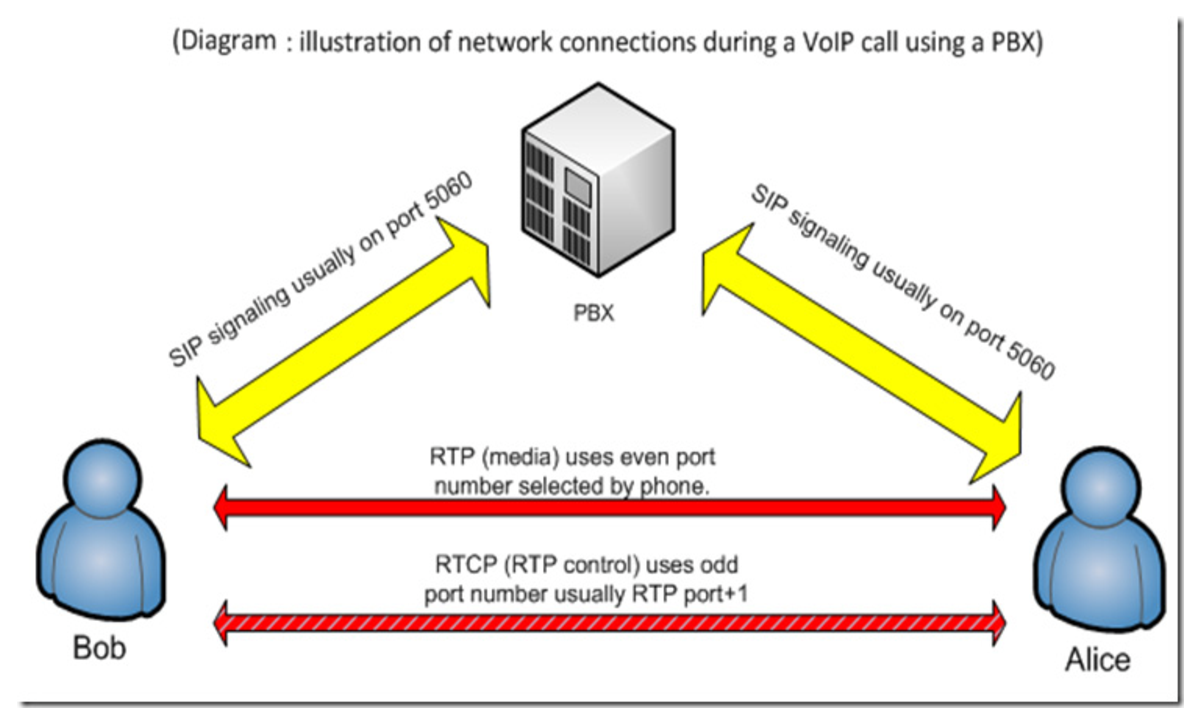
\includegraphics[width=0.9\linewidth]{images/rtp_sip}
\caption{How an RTP connection takes place for VoIP (image from \cite{rtp-sip})}
\label{fig:rtp-sip}
\end{figure}


Two flows are initialized : one for RTP and the other for RTCP. They usually use consecutive ports while RTP must use an even port number (\cite{RFC3550} Section 11). So only one pair of ports must be advertised for each host. This is only true for a unicast session. IP multicast can also be used with RTP and offer better performances if a large number of clients must access the same media resource. However, we won't give any details about how RTP multicast sessions are established since is it out of the scope of this thesis.

\subsection{RTCP}

RTP is just responsible for sending data to the receiver, with a little more information inside the packet than simple UDP. It includes sequence numbers, timestamps, information about the sources and control bits. But this mechanism alone does not give any hint about packet losses or the congestion of a link. This is why RTCP is essential in most of the applications.

According to \cite{javvin2005network}, RTCP performs four tasks : 

\begin{enumerate}
\item It provides feedback on the quality of the data distribution. It plays the role of a congestion control mechanism.
\item It carries an identifier for the RTP source called the canonical name. It allows each host to identify the participants in a particular flow. It can be useful when dealing with multicast.
\item It allows the source to compute the rate at which it has to send the packet. This takes into account the number of participants to the session.
\item It conveys minimal session control information, such as participant information to be displayed on user interface, for instance. This functionality is left optional.
\end{enumerate}

To do so, it carries Sender and Receiver reports. These reports are transmitted to the other party to estimate the quality of the link. They include information such :

\begin{itemize}
\item Packet count, octet count (received/sent)
\item Cumulative number of packets lost and fraction lost
\item Highest sequence number received
\item Different timestamps to estimate RTT and jitter.
\end{itemize}


\section{MPRTP}

Currently, RTP cannot support multipath because it operates at the session level and not at the transport level. Therefore RTP deals only with a particular media flow and not with the 5-tuple. The idea of MPRTP is to use multiple RTP flows concurrently on multiple interfaces. Figure \ref{fig:mprtp-concept} presents the system overview. As for RTP, the communication of the media is unidirectional : from a sender to at least one receiver. 


\begin{figure}
\centering
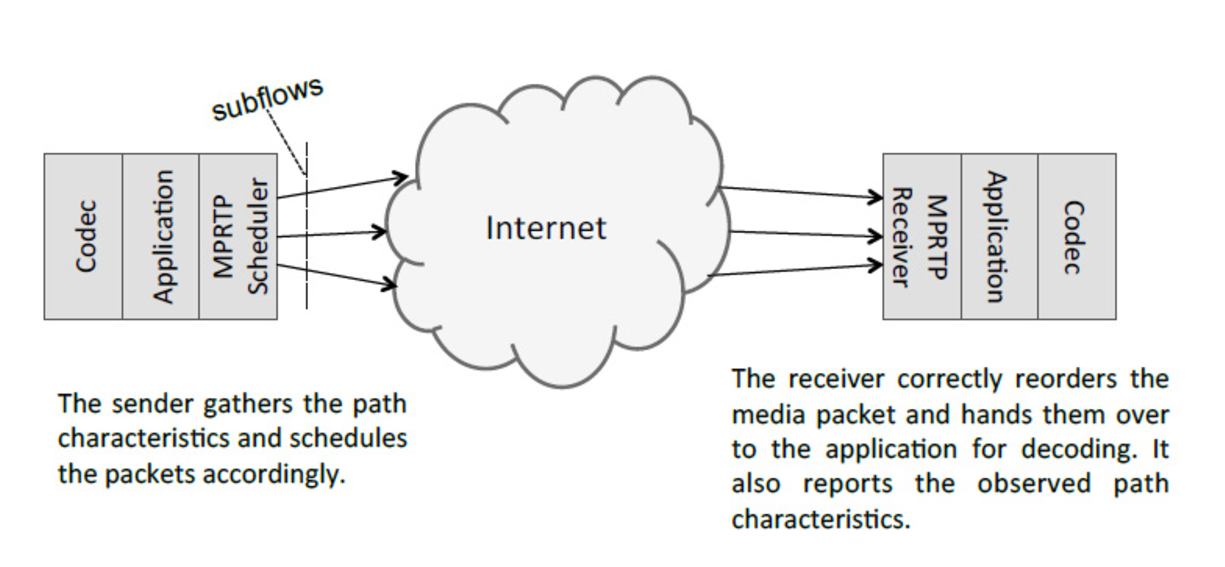
\includegraphics[width=0.9\linewidth]{images/mprtp}
\caption{MPRTP overview (taken from \cite{singh2013mprtp})}
\label{fig:mprtp-concept}
\end{figure}

\subsection{Design goals}

\subsubsection{Adapting to bandwidth changes}

If a link is congested, the scheduler must reduce the number of packets on this link and re-distribute the load among less congested links. But a small quantity of traffic must still be sent through this link just to monitor the link's characteristics (RTT, jitter). A similar approach is used in Multipath TCP \cite{wischik2011design}. Of course, the changes of repartition among the flows must be smooth and absorb small perturbations. Especially when used with mobile phones, the change of antenna may introduce a loss of connection on a very short period of time.

\subsubsection{Overcoming packet skew}

When you use disjoint paths over the Internet, you will likely encounter different delays. As a consequence, the packets will arrive out of order. To solve this problem, you need a large enough buffer at the receiver side. For multimedia communications, this is critical, as you want your song or video to be read in-order. While the problem can exist with DTLS, the constraint is less critical since the application must cope with out-of-order packets and implement by itself a buffer if needed. However, the scheduler could take care of carefully selecting the flow in order to minimize the skew.

\subsubsection{Choosing transmission paths}

Among the available paths, the MPRTP implementation must choose a subset of them to send the packets. This choice is actually an optimization problem based on multiple parameters. An endpoint may chose to optimize some of them. Following the scenario and the application needs, the scheduler may minimize losses, minimize latency or maximize end-to-end capacity.

\subsection{Getting subflow information}

To meet these goals, a scheduler will need to have information about the different sub-flows. Thanks to the sender and receiver reports from RTCP, MPRTP already have information about the complete session. However to get per-subflow information, it introduces RTCP per-subflow reporting. In order to decouple the subflow from the session, a subflow ID is assigned to each subflow. A flow is considered unique if the source and destination IP addresses and ports are different, which, together with the protocol, gives a 5-tuple.

To get an estimation of the packet jitter, packet loss and packet discard for a specific subflow, a subflow-specific sequence number is introduced. This new sequence number and the subflow ID are both carried in a header extension. This additional header is standardized in \cite{RFC3550} and will therefore allow backward compatibility.

Note that we don't have such tools in DTLS to evaluate a link's characteristics. We have build our own mechanism of feedback which is a simplified version of the sender and receiver reports of RTCP. More details are given on Section \ref{sec:mpdtls-feedback}. This extension has been designed without the multipath aspect in mind and thus could be implemented separately from MPDTLS.

\subsection{Addresses advertisement}
\label{sec:mprtp-advertise}

To establish new paths, a mechanism must advertise the addresses to the other host. In MPRTP, the choice is currently \cite{singh-avtcore-mprtp} left to the application to use in-band or out-of-band communication to take care of it.

\addtypes{byte, uint16}
\begin{lstlisting}[caption=MPRTCP Interface Advertisement, label=lst:mprtcp-advertisement]
struct {
   byte MPRTCP_Type;
   byte block_length;
   uint16 RTP_port;
   byte InterfaceAddress[(block_length-1)*4];
 } MPRTCPInterfaceAddress;
\end{lstlisting}

We focused on in-band communication since that is the way we choose to do it in our proposed design (see Section \ref{sec:advertise}). The MPRTCP extension for interface advertisement is defined in \cite{singh-avtcore-mprtp} sec. 9.3. The structure used to carry one particular IP address and port is shown on Listing \ref{lst:mprtcp-advertisement}.

The \texttt{MPRTCP\_Type} indicates the type of interface address. For now, 3 types are defined: 
\begin{enumerate}
\item IPv4 address
\item IPv6 address
\item DNS name
\end{enumerate}

The \texttt{block\_length} is the size of the block (i.e. the whole structure) in words of 32-bit. For an IPv4 address it should be 2 (1 for the interface itself and 1 for the information before), for an IPv6 it should be 5 and for a DNS name it will be variable.

The \texttt{RTP\_port} must be a valid RTP port number different from 0. The \texttt{InterfaceAddress} contains the actual IP address and its size is determined by the \texttt{block\_length}.

Note that Listing \ref{lst:mprtcp-advertisement} only presents the block to advertise one interface but such blocks will be combined in a unique packet to take into account multiple interfaces.

As stated in the working draft, all the interfaces in use must be transmitted. Moreover an endpoint must advertise its interfaces whenever an interface appears or disappears and when it receives an Interface Advertisement. We will use a similar strategy for MPDTLS. The fact you have to reply to an Interface Advertisement provides somehow an acknowledgment mechanism that could be useful in an unreliable protocol.

\subsection{Scheduling Algorithm}

The scheduler is one of the most important aspect and a critical point if you want the multipath approach to overcome the single path one. In the case of MPRTP, the sender must choose on which path to send the packets in order to guarantee a constant bit rate. A simple example with two paths is shown on Figure \ref{fig:mprtp-scheduler}.

\begin{figure}[!h]
\centering
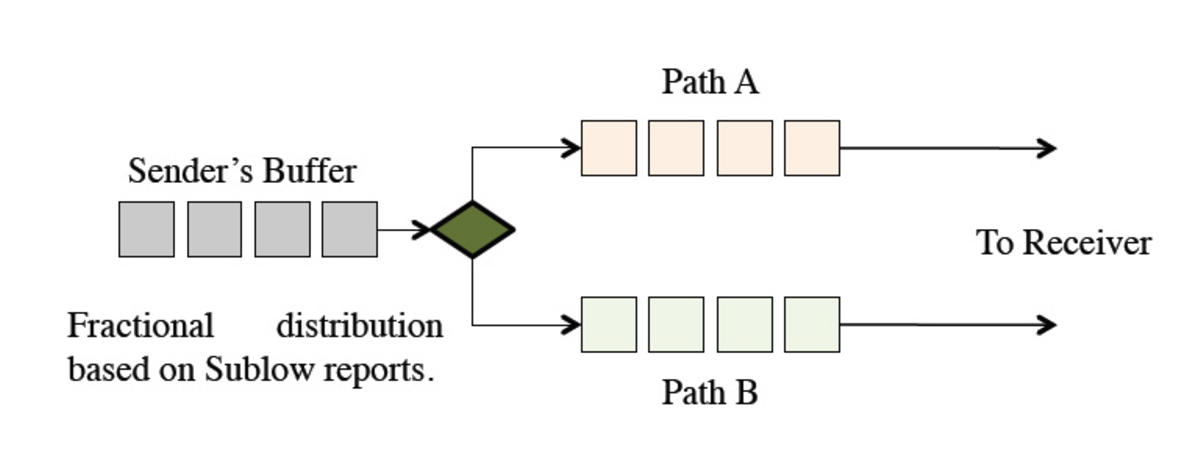
\includegraphics[width=0.9\textwidth]{images/mprtp-scheduler}
\caption{MPRTP Sender's Scheduler}
\label{fig:mprtp-scheduler}
\end{figure}

The goal of the scheduler is to compute the fractional distribution to distribute packets accordingly to paths characteristics. This means that a link with a smaller RTT will be probably given more load than another one.

However, the packets may arrive out-of-order if a significant difference in terms of RTT is noticed between paths. To compensate this reordering, a dejitter buffer must be set up at the receiver's side (Figure \ref{fig:mprtp-dejitter}). The buffer must be large enough to compensate variation in per path RTT.

\begin{figure}[!h]
\centering
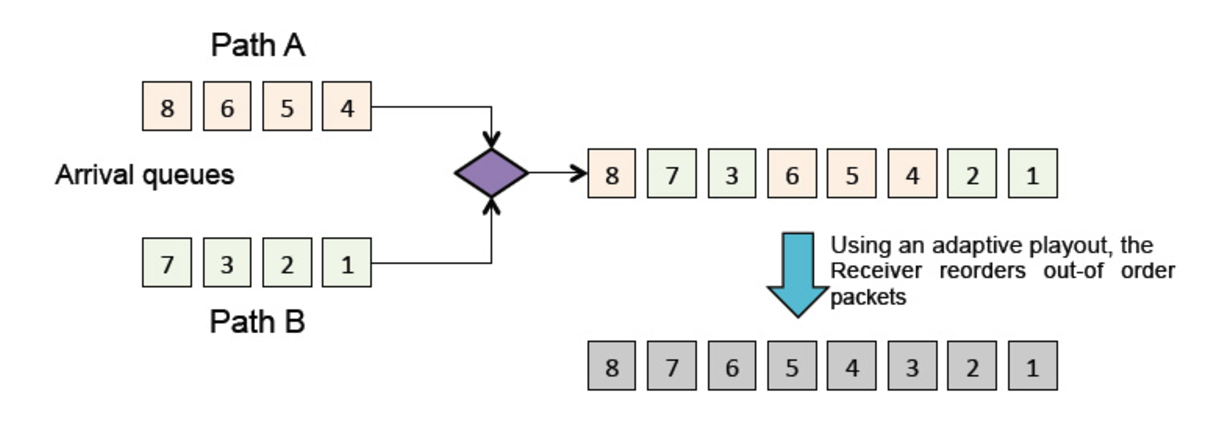
\includegraphics[width=0.9\textwidth]{images/mprtp-dejitter}
\caption{MPRTP buffer at receiver's side}
\label{fig:mprtp-dejitter}
\end{figure}

This buffer will rearrange the packets to put them in order and deliver the information to the application as a single stream.

\subsubsection{Receiver rate}

The receiver rate (RR) is computed for every flow as the total number of bytes that have been transiting through the flow between two consecutive receiver reports. This rate takes into account only the packets well received by considering the loss rate. When the receiver builds its $i^{th}$ report, the RR is computed as follow :

\begin{equation*}
RR = \frac{(\sum_{k = HSN_{i-1}}^{HSN_i} sizeof(X_k)) \times (1 - L_i)}{(t_i - t_{i-1})}
\end{equation*}

Where $HSN_i$ stands for the "Highest Sequence Number" received in the report $i$. So the sum actually represents the total number of bytes sent between two consecutive receiver reports. $L_i$ is the loss rate reported for this period of time.

\subsubsection{Calculating the fractional distribution}

The computation of the fractional distribution is not done each time the sender receives a receiver report. An interval timer is instead defined to do it more or less frequently following the network information. This interval expressed in seconds is computed as follow : 

\begin{equation*}
\begin{split}
SchInt & = \lambda \times S_{interval},\quad 0.5 \le \lambda \le 1.5 \\
 \lambda & = 0.5 + Rand(0.0,1.0)
\end{split}
\end{equation*}

The randomisation factor $\lambda$ is used to prevent multiple senders using the same paths to launch the computation as the exact same time. This would lead to a delta in server load. $S_{interval}$ is a value between the minimum and maximum RTCP interval [32,39]. It will be kept small at the beginning of the communication to recompute the distribution more frequently but progressively increases to the maximum. If congestion is detected, the $S_{interval}$ is reduced to recover quickly if the link becomes non-congested later on.

After the end of the interval, the distribution needs to take into account the state of each link in terms of congestion. For this purpose, three categories are defined : congested, mildly-congested and non-congested. To determine the category of one particular flow, the rules defined in \cite{ietf-avtcore-rtp-circuit-breakers} are used. This Internet draft aims at providing concrete rules to determine if a RTP application must stop sending packets to avoid congestion.

The proposed algorithm to split the traffic among all available paths will take into account the degree of congestion and will reduce the load of congested links.

\begin{align*}
SB[i] & = min\left( \frac{RR[i]}{\sum_{m} RR[m]} \times MR,\quad \alpha \times RR[i] \right) &\quad \text{if congested} \\
SB[i] & = min\left( \frac{RR[i]}{\sum_{r} RR[r]} \times MR,\quad \beta \times RR[i] \right) &\quad \text{if mildly-congested} \\
SB[i] & = \left( \frac{RR[i]}{\sum_{w} RR[w]} \times (MR - AP) \right) & \quad \text{if non-congested}
\end{align*}

Where $SB[i]$ is the sending bit rate for a particular path $i$, MR is the media rate (i.e. total bit rate) and $AP$ is the allocated bit rate. The indexes $m,r,w$ are used to represent the set of paths congested, mildly-congested and non-congested respectively. The minimum function is here to limit the maximum usage of a congested link but will not change anything if the link is already underused. Of course, this should be repeated for every path $i$.

The parameters $\alpha$ and $\beta$ must be tuned by experiments. In section 5.1 of \cite{singh2013mprtp}, $\beta$ is set to $0.8$ and $\alpha$ to $0.5$ after a series of tests in various configurations. These values make the scheduler reach the optimum fractional distribution quicker than other values.